\chapter{Evaluation}\label{sec:new_models}
The \gls{cnn} analyzed in Section~\ref{sec:classifier} is going to be taken as a starting point to build \textbf{new models}. These models will be trained with \textbf{different datasets} and \textbf{regularization methods} and, finally, \textbf{new architectures} will be implemented. In this chapter, the tools developed in Section~\ref{sec:bencharmk} will be employed to evaluate the results achieved by each \gls{cnn}. Before talking about the performance of the new models, the visualization of the convolutional layers filters and activation maps is going to be analyzed.

\section{Convolutional layers visualization}
The filters and activation maps discussed in the following sections belong to the convolutional layers of the \textit{0-1; Patience=2} model that can be found in Section~\ref{sec:early_stopping}. This model has been trained with the \textit{0-1} dataset (see Section~\ref{subsec:handmade}) and an early stopping rule with patience 2. Its architecture corresponds to the one defined in Section~\ref{sec:understanding}.

\subsection{Filters}
When loading the weights of the \textbf{first convolutional layer}, a Numpy array of shape (1, 3, 3, 32) is obtained. This means that the weights are arranged in 32 filters of size 3x3. In this case, the input is a grayscale image, so the filters only have one channel (i.e. depth=1). Besides that, when examining their values, \textbf{negative and positive coefficients} are found.

In Figure~\ref{fig:filters}, these filters are plotted. Some of the filters look too noisy to tell which kind of feature they are looking for. However, a few of them can be interpreted as folllows:
\begin{itemize}
	\item \textbf{Horizontal edges}: filters 7, 9 and 23.
	\item \textbf{Vertical edges}: filters 8, 15 and 31.	
\end{itemize}

\begin{figure}
	\centering
	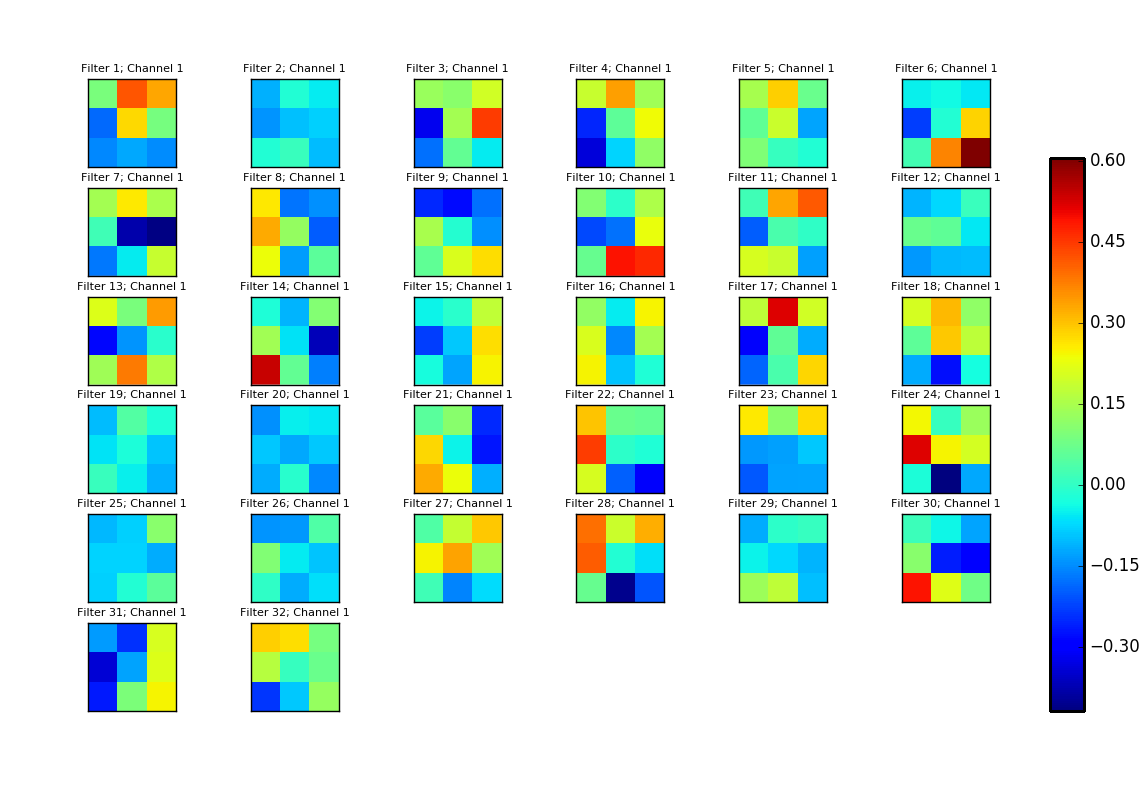
\includegraphics[width=0.85\linewidth, keepaspectratio]{figures/weights_conv2d_1.png}
	\caption{Filters of the first convolutional layer.}
	\label{fig:filters}
\end{figure}

The filters in the \textbf{second convolutional layer} have been displayed as well. The shape of the weights in this layer is (32, 3, 3, 32), which means that there are 32 filters with size 3x3. This time, its depth is 32, since there is one channel per activation map generated by the previous layer. As we get \textbf{deeper in the \gls{cnn}} and the dimensionality grows, the filters look noisier and become harder to interpret, as it can be seen in Figure~\ref{fig:filters2}.
\begin{figure}
	\centering
	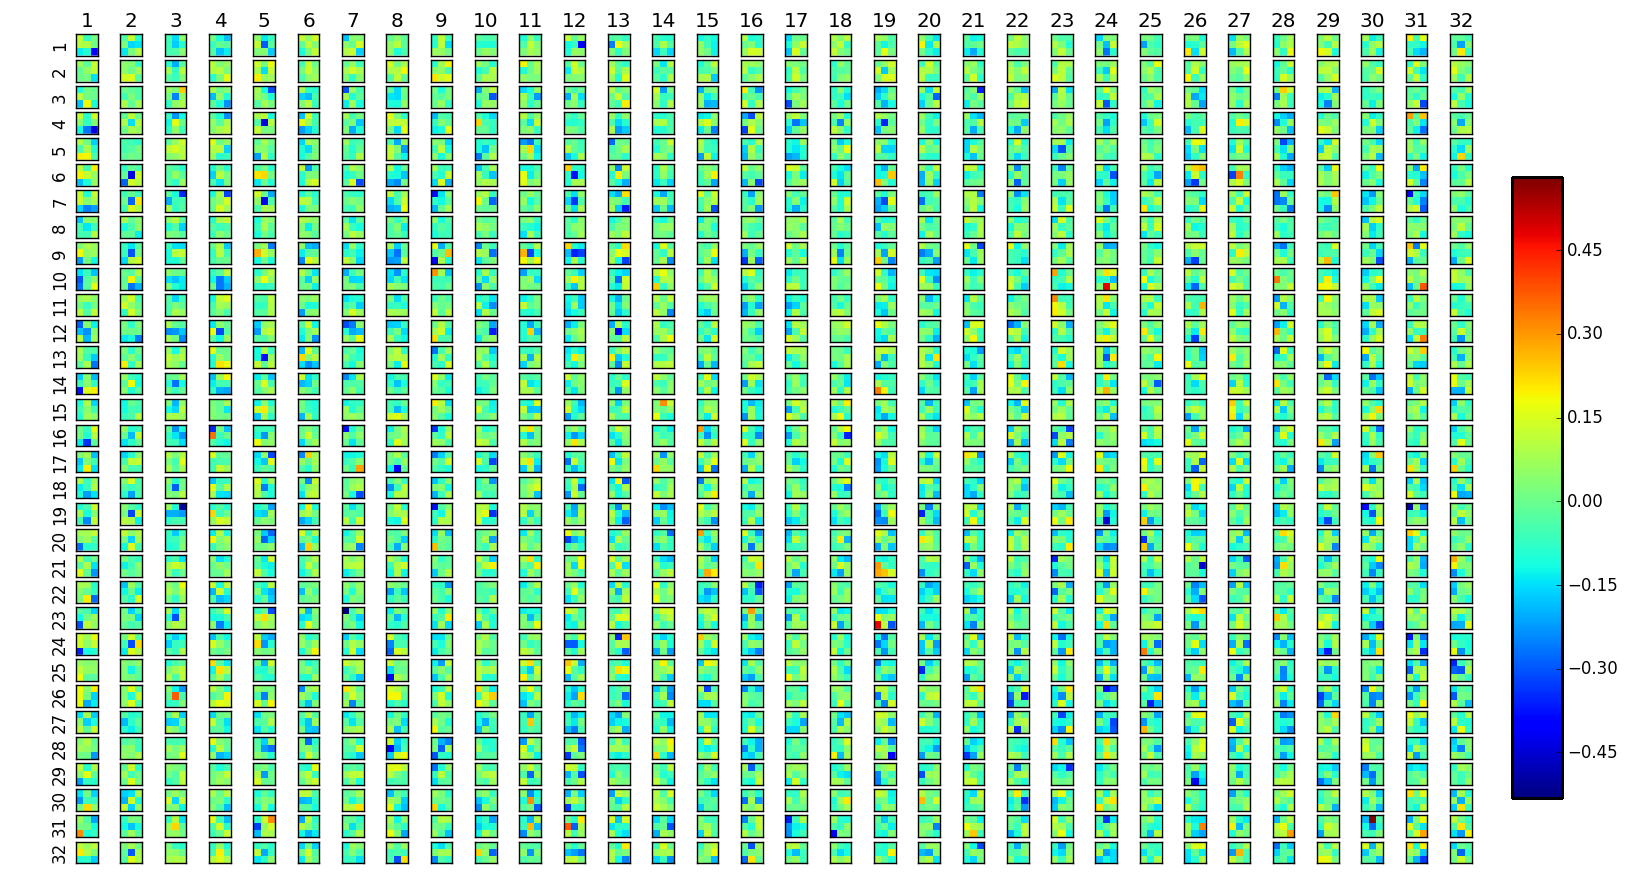
\includegraphics[width=1\linewidth, keepaspectratio]{figures/weights_conv2d_2.png}
	\caption[Filters of the second convolutional layer.]{Filters of the second convolutional layer. Each row contains the channels (1-32) that correspond to each filter (1-32).}
	\label{fig:filters2}
\end{figure}

\subsection{Activation maps}
Figure~\ref{fig:activation_maps} shows the activation maps that the \textbf{first convolutional layer} of the model outputs. There are \textbf{horizontal and vertical edge images} that confirm the interpretation of the filters given in the previous section. Besides that, some activation maps (2, 12, 19, 25 and 26) look \textit{dead}. If we look back into Figure~\ref{fig:filters}, these activation maps correspond to filters with \textbf{almost flat coefficients}. This may be a signal of a high learning rate~\cite{cs231n}. In this case, the learning rate is not explicitly declared: the ADADELTA optimizer \ref{adadelta} use an adaptive one.
\begin{figure}
	\centering
	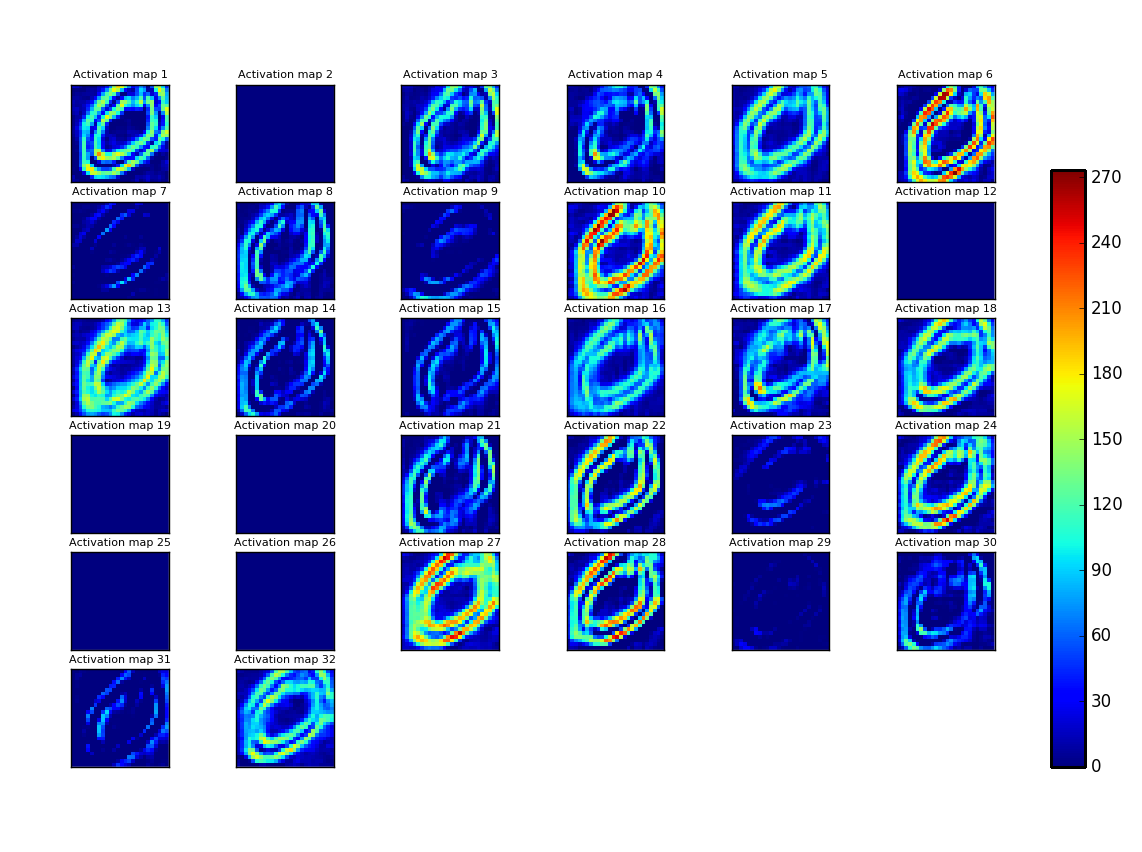
\includegraphics[width=0.85\linewidth, keepaspectratio]{figures/activation_maps_conv2d_1.png}
	\caption{Activation maps of the first convolutional layer.}
	\label{fig:activation_maps}
\end{figure}

The activation maps of the \textbf{second layer} are shown in Figure~\ref{fig:activation_maps2}. The images obtained look \textbf{more specialized} than the ones in the previous layer. It's easier to tell to what kind of feature (e.g. edges and corners) each activation map is responding to.
\begin{figure}
	\centering
	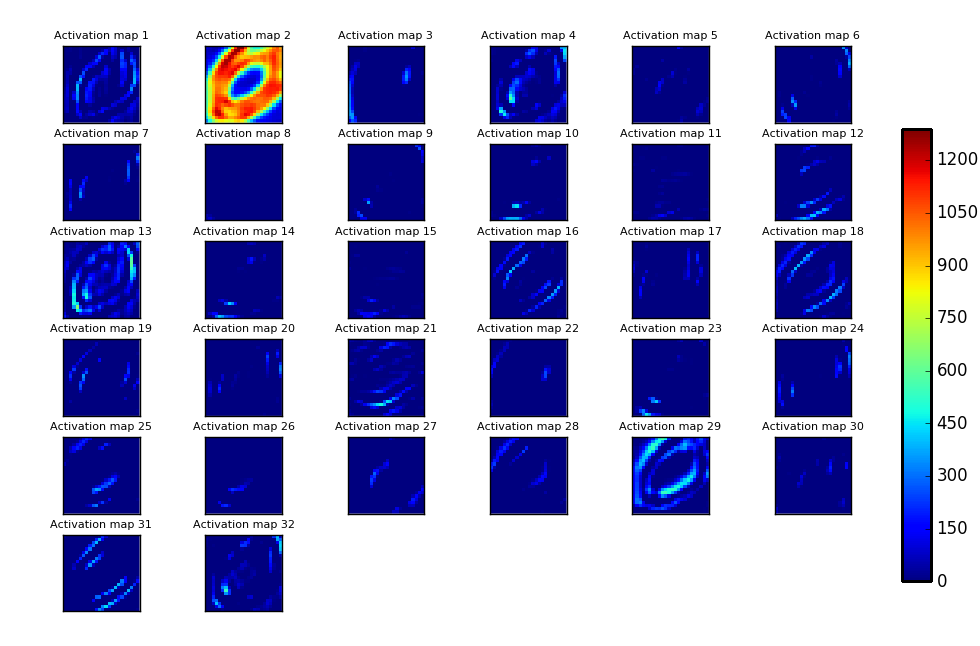
\includegraphics[width=0.85\linewidth, keepaspectratio]{figures/activation_maps_conv2d_2.png}
	\caption{Activation maps of the second convolutional layer.}
	\label{fig:activation_maps2}
\end{figure}

It's important to note that the values of the activation maps are \textbf{always positive}, even if the filters have negative coefficients. This is because the \gls{relu} activation function (see Equation~\ref{eq:relu}) turn all the negative values to zero.

\section{New datasets}\label{sec:new_datasets}
The original model has been trained with each of the \textbf{handmade datasets} described in Section~\ref{sec:datasets}. The number of epochs has been set to 12 and the evaluation has been carried out with the \textbf{1-6 test dataset}. The results that can be seen in Table~\ref{tbl:datasets} lead to the following conclusions:
\begin{itemize}
	\item As it might be expected, the results when training with the \textbf{Sobel dataset} are much worse than the ones obtained with the other datasets, because we're testing with noisy images a \gls{cnn} trained with noiseless samples.
	\item The \textbf{\textit{0-6} and \textit{1-6} models} are the ones that achieve better results, as they have been trained with \textbf{six times more samples} than \textit{0-1} and \textit{1-1}.
	\item When \textbf{comparing \textit{0-1} with \textit{1-1} and \textit{0-6} with \textit{1-6}}, it can be seen that the performance is almost the same, which means that the \textbf{gradient image without noise and transformations} is not adding much information to the model.
\end{itemize}

Taking all of this into account, it has been decided to keep working with the \textbf{\textit{0-1} model}, which achieves a performance that is comparable with the other models with the advantage of a much lower computational cost.

\begin{table}
	\centering
	\begin{tabular}{l*{4}{c}r}
		\textbf{Model} & \textbf{Loss} & \textbf{Accuracy} & \textbf{Epochs} \\
		\hline
		Sobel & 1.233 & 0.699 & 12 \\
		0-1 & 0.201 & 0.939 & 12 \\
		1-1 & 0.189 & 0.943 & 12 \\
		0-6 & 0.109 & 0.968 & 12 \\
		1-6 & 0.111 & 0.967 & 12 \\
	\end{tabular}
	\caption{Results of training with different datasets.}
	\label{tbl:datasets}
\end{table}

\section{Regularization methods}
"\textbf{Regularization} is any modification we make to a learning algorithm that is intended to reduce its \textbf{generalization error} but not it's \textbf{training error}"~\cite{Goodfellow-et-al-2016}. Reducing the generalization error is important because, even if a model achieves a great accuracy or loss with the training dataset, if it doesn't generalize well enough, the results during validation and test time won't be optimal. This is specially significant in our case, since the predictions of the digit classifier will be based on \textbf{images that differ a lot from the train dataset}. In this section, the effect of applying to the \textit{0-1} model two regularization techniques (\textbf{early stopping} and \textbf{dropout}) is going to be evaluated. 

\subsection{Early stopping}\label{subsec:early_stopping}
The models in the previous section have been trained for 12 epochs. However, if we look at the \textbf{validation results} in Figure~\ref{fig:val_datasets}, the models were \textbf{not overfitting} yet, because the results didn't stop improving. This means that they were not being trained as much as possible. Setting an early stopping rule (see Section~\ref{subsec:callbacks}) allows training the \gls{cnn} right until it starts to overfit, making the most of it. The criteria that has been used depends on the loss during validation. The model is trained until the log-loss (see Section~\ref{eq:categorical_crossentropy}) has not improved after two validations in a row, i.e. a patience of 2. Besides that, in order to keep the best \textit{version} of the model, the log-loss is checked after each epoch and if it's the lower than the previous best log-loss achieved, the weights of the model are saved, overwritting the weights of the previous best \textit{version}. The difference between training the model with and without early stopping can be seen in Table~\ref{tbl:earlystopping}.
\begin{figure}
	\centering
	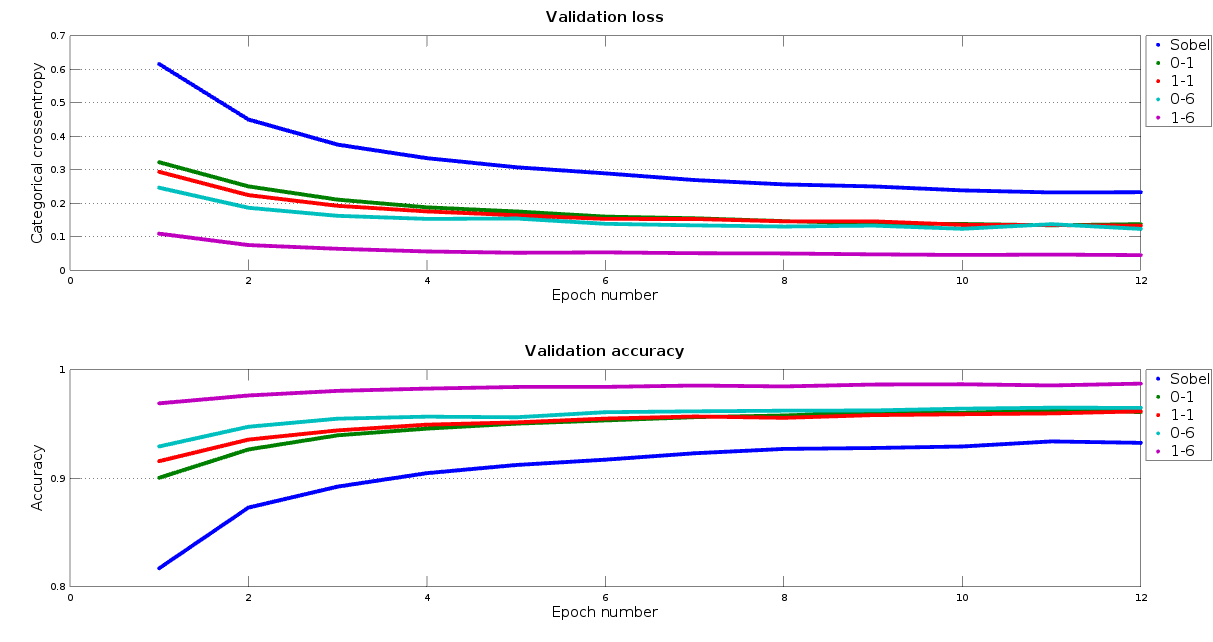
\includegraphics[width=1\linewidth, keepaspectratio]{figures/val_datasets.png}
	\caption{Validation results when training the model with different datasets.}
	\label{fig:val_datasets}
\end{figure}

\begin{table}
	\centering
	\begin{tabular}{l*{4}{c}r}
		\textbf{Model} & \textbf{Loss} & \textbf{Accuracy} & \textbf{Epochs} \\
		\hline
		0-1 & 0.201 & 0.939 & 12 \\
		0-1; Patience=2 & 0.155 & 0.954 & 30 \\
	\end{tabular}
	\caption{Results of training with and without early stopping.}
	\label{tbl:earlystopping}
\end{table}

Early stopping means an improvement of 1.6\% in accuracy and 4.6\% in log-loss. The model has been trained for 30 epochs and reached its best \textit{version} at the 27$^{th}$ epoch. Setting a longer patience has been considered, but it has been decided to apply it only to the best model obtained after Section~\ref{subsec:arch} to reduce the computational cost.

\subsection{Dropout}
The models that we're working with insert dropout (see Section~\ref{subsec:layers}) before every dense layer of the \gls{cnn} (0.25\% and 0.5\%, respectively). Dropout is usually applied just to fully connected or dense layers, because convolutional layers are less likely to overfit due to their architecture. In order to determine how dropout affects the performance of the model, the \textit{0-1; Patience 2} dataset has been trained with and without the mentioned dropout. The results can be seen in Table~\ref{tbl:dropout}. 
\begin{table}
	\centering
	\begin{tabular}{l*{4}{c}r}
		\textbf{Model} & \textbf{Loss} & \textbf{Accuracy} & \textbf{Epochs} \\
		\hline
		No dropout & 0.189 & 0.945 & 9 \\
		Dropout & 0.155 & 0.954 & 30 \\
	\end{tabular}
	\caption{Results of training with and without dropout.}
	\label{tbl:dropout}
\end{table}

Without dropout, the model has stopped training after 9 epochs. It has learned faster, but it has started overfitting earlier, resulting in worst results that the ones achieved by the model trained with dropout. This can be clearly seen in Figure~\ref{fig:comp_dropout}
\begin{figure}
	\centering
	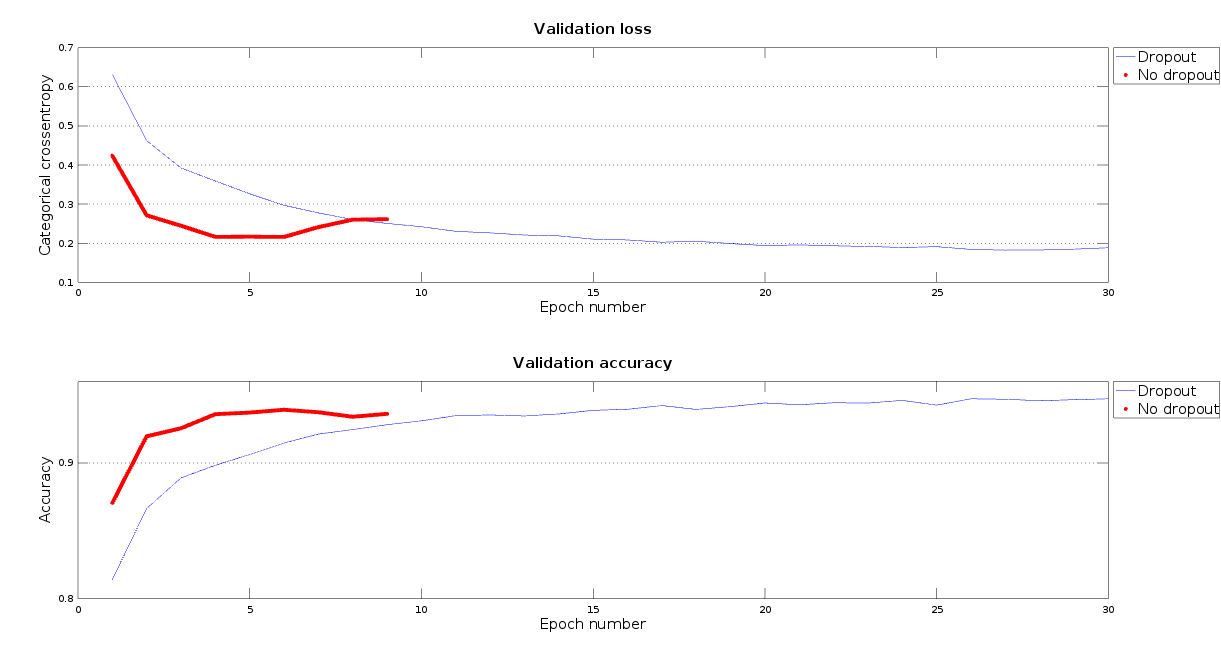
\includegraphics[width=1\linewidth, keepaspectratio]{figures/comp_dropout.png}
	\caption{Validation results with and without dropout.}
	\label{fig:comp_dropout}
\end{figure}

Additionally, in Figure~\ref{fig:lc_dropout}, the learning curves of the models can be seen. It's worth looking into these plots to realize that validation results are better than training results when the model is trained with dropout. This may look illogical, as the \gls{cnn} should always perform better with samples that it has already seen. However, it's important to remember that dropout only applies during training and, as it will \textit{switch off} a lot of weights in the \gls{cnn}, much of its prediction power will be lost. During validation, there are no \textit{switched off} weights, which allows the \gls{cnn} to make better predictions. Besides that, in the figure can be seen that the training results are much better (i.e. lower loss and higher accuracy) when the model is trained without dropout, while the validation results are better with dropout. This means that the model with dropout is generalizing better than the one without dropout. 
\begin{figure}
	\begin{subfigure}{1\textwidth}
		\centering
		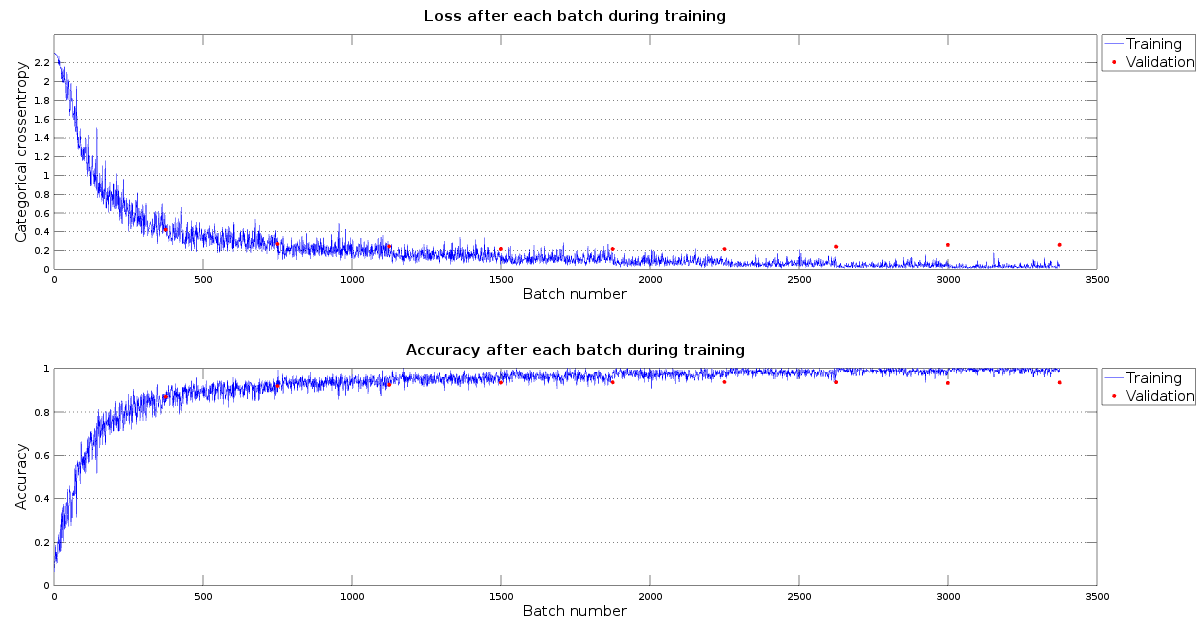
\includegraphics[width=1\linewidth]{figures/lc_nodropout.png}
		\caption{Learning curves without dropout.}
	\end{subfigure}
	\begin{subfigure}{1\textwidth}
		\centering
		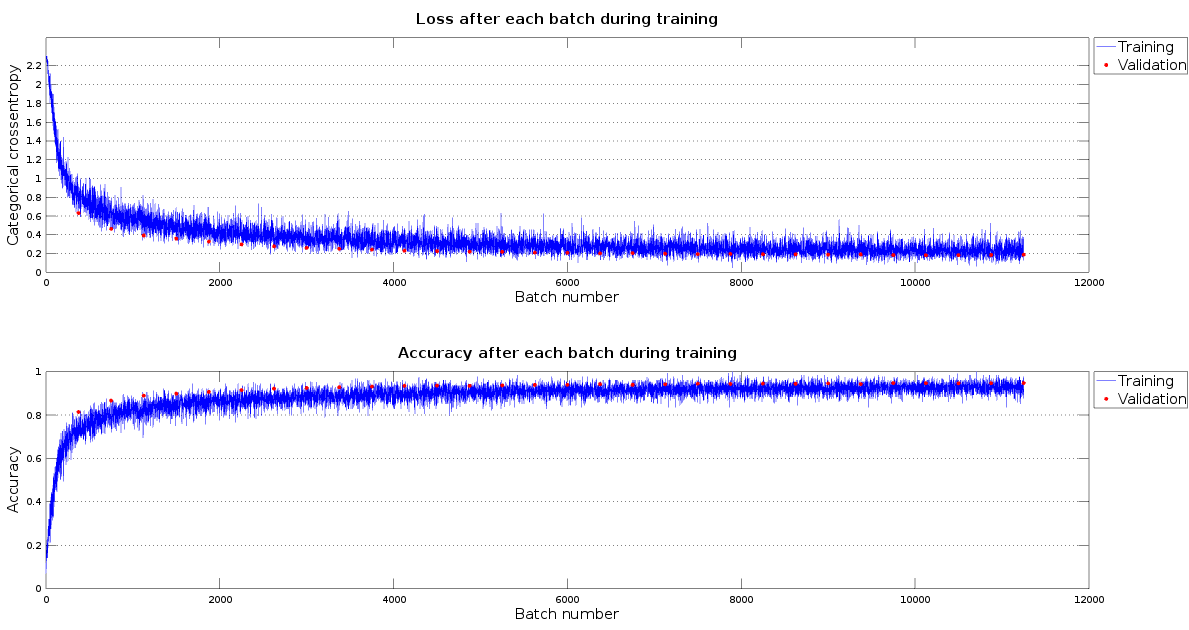
\includegraphics[width=1\linewidth]{figures/lc_dropout.png}
		\caption{Learning curves with dropout.}
	\end{subfigure}
	\caption[Learning curves with and without dropout.]{}
	\label{fig:lc_dropout}
\end{figure}

\section{New architectures}\label{subsec:arch}
In order to check the influence of different architectures in the performance of the \gls{cnn}, new models with a different number of convolutional layers have been trained and tested. The stopping rule used in these trainings is the one defined in the previous section and dropout is also applied. The decision of adding pooling layers to the models (see Section~\ref{subsec:layers}) has been taken to reduce computational cost. In the first attempt at training a model with 6 convolutional layers, I triplicated the model with 2 convolutional layers and one MaxPooling layer. However, a MaxPooling layer was removed because the model ended up working with an empty image: 0x0 size.
\begin{table}
	\centering
	\begin{tabular}{l*{4}{c}r}
		\textbf{Model} & \textbf{Loss} & \textbf{Accuracy} & \textbf{Epochs} \\
		\hline
		1Conv+MaxPooling & 0.191 & 0.945 & 47 \\
		2Conv+MaxPooling & 0.155 & 0.954 & 30 \\
		3Conv+MaxPooling & 0.129 & 0.945 & 28 \\
		2Conv+MaxPooling+2Conv+MaxPooling & 0.092 & 0.970 & 27 \\
		4Conv+MaxPooling+2Conv+MaxPooling & 0.092 & 0.971 & 24 \\
	\end{tabular}
	\caption{Results of training models with different architectures.}
	\label{tbl:arch}
\end{table}

As it can be seen in Table~\ref{tbl:arch}, the best results have been obtained with the models that contain 4 and 6 convolutional layers. Besides that, taking a look into the validation curves (see Figure~\ref{fig:comp_arch}), it can be assumed that when we increase the number of layers, the neural network tends to lead to better results with less epochs.

\begin{figure}
	\centering
	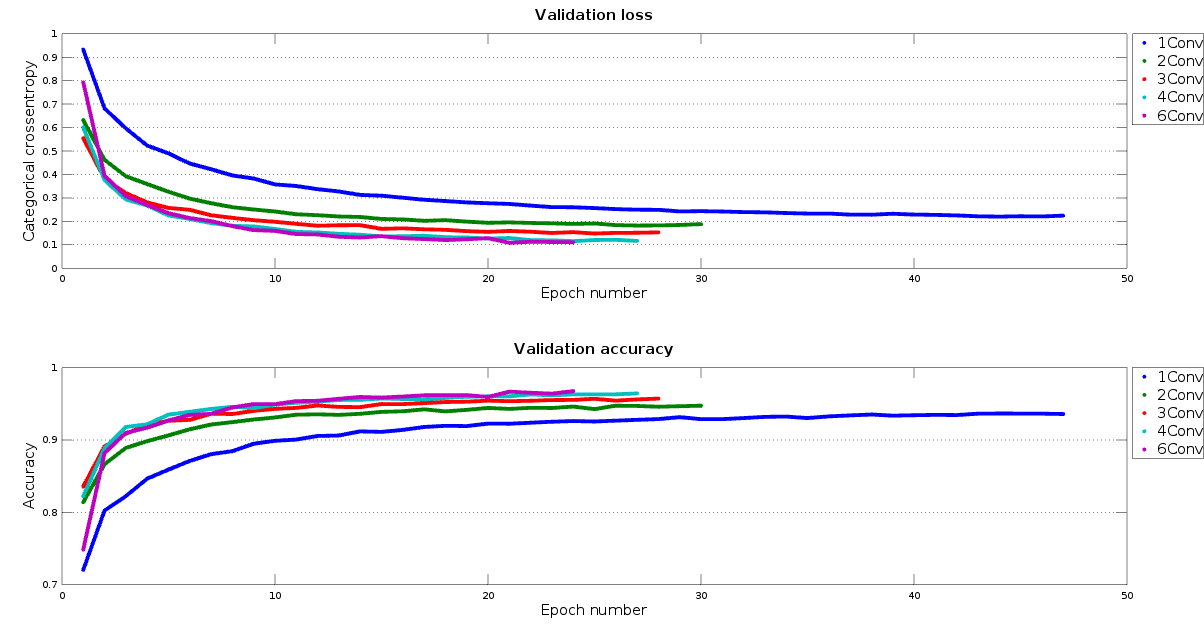
\includegraphics[width=1\linewidth, keepaspectratio]{figures/full_comparison.png}
	\caption{Validation results with different architectures.}
	\label{fig:comp_arch}
\end{figure}

The model with 6 layers has a slightly better accuracy but a slightly worse loss than the one with 4 layers. Considering that computational cost is higher when training the \textit{6Conv} model, \textit{4Conv} model seems to be the best bet. In order to make the most of it, it has been trained again but increasing the patience of the early stopping from 2 to 5. The results obtained with the new stopping rule can be seen in Table~\ref{tbl:arch_patience5}. These results imply that being more \textit{patient} during training can lead to a better performance, although in this case the improvement is not very significant.
\begin{table}
	\centering
	\begin{tabular}{l*{4}{c}r}
		\textbf{Model} & \textbf{Loss} & \textbf{Accuracy} & \textbf{Epochs} \\
		\hline
		4Conv; Patience=2 & 0.092 & 0.970 & 27 \\
		4Conv; Patience=5 & 0.082 & 0.973 & 37 \\
	\end{tabular}
	\caption{\textit{4Conv} model trained with different stopping rules.}
	\label{tbl:arch_patience5}
\end{table}